\documentclass[a4paper]{article}

\usepackage[utf8]{inputenc}	% Flere sprog tegnsæt (fx æøå)
\usepackage[english]{babel}	% Dansk orddeling (kan ændres til english)
\usepackage[T1]{fontenc}		% Brug 8-bit front
\usepackage{lmodern}		% Vektor front

\usepackage{02459}

\usepackage[svgnames]{xcolor} % Udvider \color med "SVG color names"
\usepackage{graphicx}	% Kompatibilitet til visning af pixel billeder (.png, .jpg, .gif)
\usepackage{epstopdf}	% Kompatibilitet til visning af vector billeder (.eps)
\usepackage{parskip}	% Tilføjer vertikal margin til hver paragraph
\usepackage{float}		% TIllader H som positions parameter
\usepackage{subcaption}	% Tillader subfigure, subtable samt \captions
\usepackage{amssymb}	% Flere matematiske symboler
\usepackage{amsthm}      % Endnu flere matematiske symboler
\usepackage{mathtools}	% Det meste matematik (indeholder ams­math og rettelser)
\usepackage{xfrac}		% Flere fracs (\sfrac{}{})
\usepackage{listings}	% Indsæt code
\usepackage{algorithm}
\usepackage[noend]{algpseudocode}
\usepackage{todonotes}	% Cool to-do notes, [disable] skjuler to-do
\usepackage[bookmarks,bookmarksnumbered,hidelinks]{hyperref} % clickable pdf (til sidst)
\usepackage[bibstyle=ieee,citestyle=numeric-comp]{biblatex} % Benyt BibLaTeX til formatering
\usepackage{cleveref} % \cref's (has to be the last loaded ref. package)

\setlength{\marginparwidth}{80pt} 				% Mere brede på margin notes og to-do
\setlength{\parindent}{0cm}   					% Deaktiver afsnit indrykning
\DeclareGraphicsExtensions{.pdf,.eps,.png,.jpg,.gif}
\numberwithin{equation}{section}

\addbibresource{bibliography.bib}

\begin{document}

\title{Convolutional Neural Networks and Algebraic Scale Invariance \\ for Speech Classification}
\name{Andreas Madsen (s123598), Frederik Wolgast Rørbech (s123956), Lasse Regin Nielsen (s123815)}
\address{Technical University Of Denmark}
\date{\today}

\maketitle

% Using input because of page restriction of 4 pages (\include adds newpage)
%!TEX root = main.tex
\begin{abstract}
In a recent paper by Dieleman et al \cite{dieleman}, a convolutional neural network is used for end-to-end learning in music. In this paper the network is applied to sex and speaker classification and shown to have varying degrees of success. Inspired by an earlier paper by Yann Le Cun et al \cite{scale-invariante}, a special regularizer ensuring scale invariance, with the idea being that models should be invariant to small perturbations of input, is implemented but ultimately does not  improve model performance. 

\end{abstract}

% USE: http://www.ieee.org/documents/taxonomy_v101.pdf
\begin{keywords}
feature learning, convolutional neural network, speaker recognition, regularization, invariance
\end{keywords}
%!TEX root = main.tex
\section{Introduction}

Traditionally a two-stage approach of first feature extraction and secondly inputting these feature into a classifier, have been used for speaker classification. An example of such is a model using MFCC features and then fitting an GMM to each speaker.

Getting these feature right requires a wast amount of domain knowledge. Resent effort \cite{dieleman} in neural networks, have shown that it is possible to use a simple spectogram and a convolutional neural network to produce similar results on a tag classification problem.

In this paper the performance of the Dieleman \cite{dieleman} network on the speakers classification problem is investigated. Finally since it was found that the Dieleman network didn't experience any performance gain from using regularization\cite{dieleman}, we will create a special regularizer that should cause the model to become scale invariant. This regularizer is inspired from \cite{scale-invariante} and specialized for scale invariance.

%!TEX root = main.tex
\section{Materials and Methods}

\subsection{Datasets: ELSDSR and TIMIT}

Two datasets were used for speaker classification; ELSDSR and TIMIT. The ELSDSR dataset includes 23 people and was specifically created for automatic speaker recognition. The TIMIT dataset is an acoustic-phonetic speech corpus and was thus not directly created for automatic speaker recognition. As a result, the TIMIT dataset has people with few observations or very short soundclips. To accommodate for this the dataset was filtered to only include people with sufficiently many long observations. After this filtering only 81 people were left.

Both datasets were preprocessed by normalizing the energy (L2 norm) of each signal to be one, and then a globally normalize the data to $\mu = 0$ and $\sigma = 1$.

\subsection{The Dieleman network}

The Dieleman network, expecting a spectrogram $x \in \mathbb{R}^{m \times n}$ as input, consists of 6 layers: 2 $\times$(\emph{Convolutional} layer + \emph{Max Pooling} layer), followed by 2 consecutive fully connected \emph{Dense} layers.

The 1st Convolutional layer contains $32$ filters (kernels) of dimension $m \times 8$. Each filter only convolutes along the time axis with a stride of $1$ computing a single value for each stride offset, resulting in an output of size $n - \frac{8}{2} + 1 = n - 3$ for each filter i.e. the output of layer 1 is of dimension $32 \times (n-3)$. This is illustrated in \cref{fig:convolution-1}.

\begin{figure}[H]
  \centering
  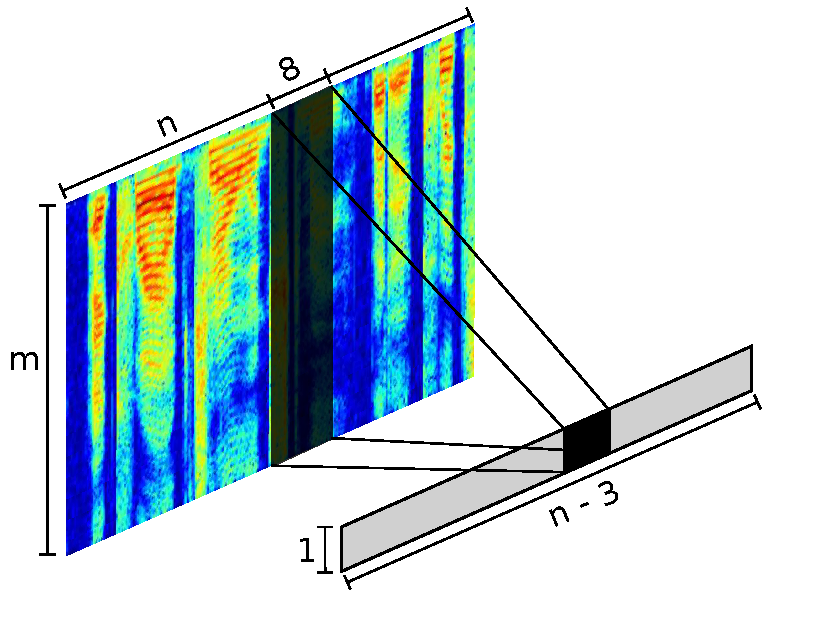
\includegraphics[width=0.4\textwidth]{inkscape/convolution.pdf}
  \caption{Illustration of 1st convolution layer for a single filter.}
  \label{fig:convolution-1}
\end{figure}

The 2nd layer performs a 1-dimensional max pooling of size $1 \times 4$ on the output from layer 1, i.e. for each filter in layer 1, a window of size $1 \times 4$ is slid through the result with a stride offset of $4$ extracting the maximum value in the window.

This reduces the dimensionality of the output by $4$, thus giving a layer output of size $32 \times \frac{1}{4}(n-3)$.

For the 3rd and 4th network layer the same procedure is applied using filters of size $1 \times 8$, and again a max pooling of size $1 \times 4$.

Finally the output of layer 4 is fed into a regular fully-connected dense layer of $100$ nodes, and then a softmax function is used as the final layer.

On the \emph{Convolutional} and \emph{Dense} layers the rectifier function (\cref{eq:rectifier}) is used as activation function
\begin{equation}
  f(x) = \text{max(}0, x\text{)},
  \label{eq:rectifier}
\end{equation}
i.e. the layers uses rectified linear units (ReLU).

The network is implemented in \texttt{python} using the library \texttt{lasagne}, which is implemented on top of \texttt{Theano} which allows for the use of highly optimized mathematical expression implementations, and also allows for transparent use of GPUs \cite{theano}.

\subsection{Scale Invariant Regularization}

The cross entropy loss function for classification is given as:
\begin{equation}
\mathcal{L}_{entropy} = - \frac{1}{N} \sum_{i=1}^N \sum_{k=1}^K t_{i,k} \ln(P(C_{i,k} | x_i, w))
\end{equation}

The approach used in \cite{scale-invariante}, is to add a transformation invariant regularizer to this loss function. The transformation is given as $s(x, \alpha)$ where $x$ is the observation and $\alpha$ is the transformation parameter. The only restriction on $s$ is that $s(x, 0) = x$. As such two examples of $s$ are:
\begin{align}
\text{scale transformation:}&\quad s(x, \alpha) = (1+\alpha) x\\
\text{offset transformation:}&\quad s(x, \alpha) = x + \alpha
\end{align}

The regularizer then penalizes changes in the output function (in this case $P(C_{i, k})$), by minimizing the derivative of the output function with respect to $\alpha$.
\begin{equation}
\mathcal{R}(s) = \frac{1}{N} \sum_{i=1}^N \left. \frac{\partial P(C_{i, k} | s(x_i, \alpha), w)}{\partial \alpha} \right|^2_{\alpha=0}
\end{equation}
By using the chain rule the derivative can be expressed as:
\begin{equation*}
\left. \frac{\partial P(C_{i, k} | s(x_i, \alpha), w)}{\partial \alpha} \right|_{\alpha=0} = \left.\nabla_x P(C_{i, k} |  x_i, w) \frac{\partial s(x_i, \alpha)}{\partial \alpha} \right|_{\alpha=0}
\end{equation*}

This is extremely convenient from an implementation perspective, as $P(C_{i, k} | x_i, w)$ is already expressed as a Theano graph. More concretely for the scale and offset invariance the regularizers become:
\begin{align}
\text{scale invariant: }& \mathcal{R} = \frac{1}{N} \sum_{i=1}^N \left(\nabla_x P(C_{i, k} | x_i, w) \bigcdot x_i\right)^2 \\
\text{offset invariant: }& \mathcal{R} = \frac{1}{N} \sum_{i=1}^N \left(\nabla_x P(C_{i, k} | x_i, w) \bigcdot \mathbf{1}\right)^2
\end{align}

The full loss function is then $\mathcal{L} = \mathcal{L}_{entropy} + \lambda \mathcal{R}$, where $\lambda$ is the regularization parameter.

%!TEX root = main.tex
\section{Results}

The Dieleman model was used for both sex and speaker classification. The results are presented below.

\begin{table}[H]
\centering
\begin{tabular}{r|c|c}
model & TIMIT & ELSDSR \\ \hline
                    Baseline & $0.354$ & $0.465$ \\
                    Logistic & $0.094 \pm 0.012$ & $0.030 \pm 0.007$ \\
                 GMM on MFCC & $0.192 \pm 0.024$ & $0.140 \pm 0.019$ \\
                    Dieleman & $0.093 \pm 0.012$ & $0.026 \pm 0.006$ \\
     Dieleman + Weight Decay & $0.114 \pm 0.013$ & $0.036 \pm 0.016$ \\
  Dieleman + Scale Invarient & $0.111 \pm 0.015$ & $0.022 \pm 0.006$ \\
 Dieleman + Offset Invarient & $0.107 \pm 0.008$ & $0.027 \pm 0.014$ \\
\end{tabular}
\caption{misclassification rate for sex classification with $95\%$ confidence internal.}
\end{table}

\begin{table}[H]
\centering
\begin{tabular}{r|c|c}
model & TIMIT & ELSDSR \\ \hline
                    Baseline & $0.988$ & $0.957$ \\
                    Logistic & $0.796 \pm 0.046$ & $0.338 \pm 0.043$ \\
                 GMM on MFCC & $0.836 \pm 0.020$ & $0.391 \pm 0.023$ \\
                    Dieleman & $0.965 \pm 0.021$ & $0.570 \pm 0.029$ \\
     Dieleman + Weight Decay & $0.944 \pm 0.020$ & $0.552 \pm 0.045$ \\
  Dieleman + Scale Invarient & $0.973 \pm 0.007$ & $0.640 \pm 0.110$ \\
 Dieleman + Offset Invarient & $0.971 \pm 0.006$ & $0.628 \pm 0.117$ \\
\end{tabular}
\caption{misclassification rate for speaker classification with $95\%$ confidence internal.}
\end{table}

As seen the Dieleman model does not appear to be better than a simple logistic model or the GMM. Because the logistic model can be expressed as a simple neural network, we attempted to expand the logistic network with individual layers form the Dieleman network, however all configuration that uses convolutional layers performed performed similarly to the Dieleman network.

Because the Scale Invariant and Offset Invariant regularizers did not improve the results on sex or speaker classification, the regularizers under optimal conditions. These conditions are synthetically constructed 2 dimensional datasets. \todo{elaborate}

\begin{figure*}[h]
	\centering
	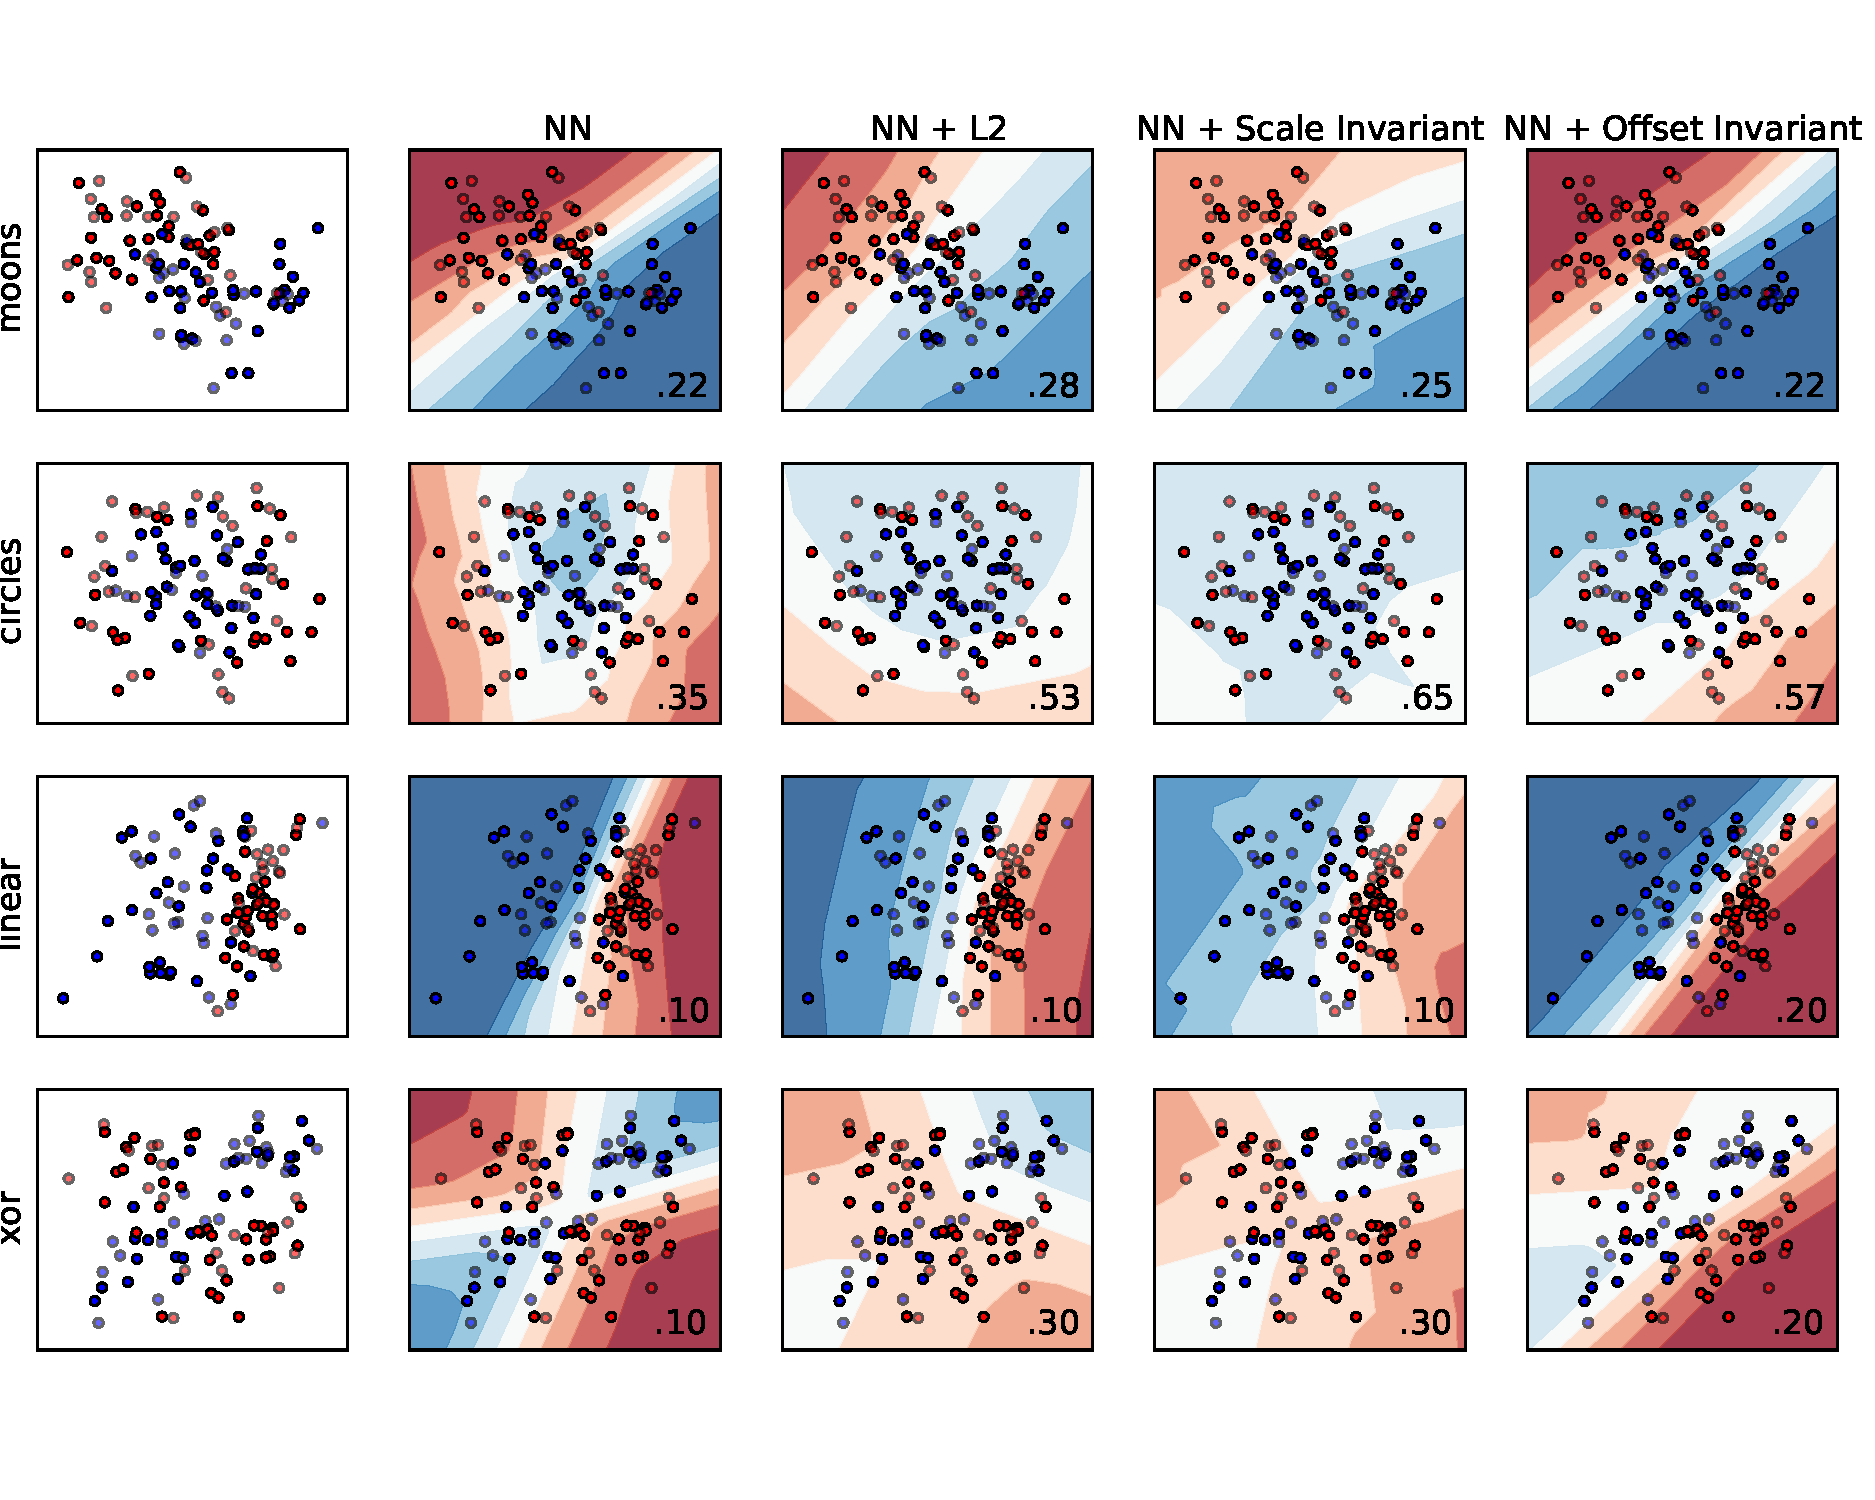
\includegraphics[width=0.7\textwidth, trim = 0 2.2cm 0 2cm, clip]{plots/2d_classifier}
	\caption{Observations and contour plot of the class probability function for each classifier and dataset.}
\end{figure*}

100 datasets for each data generator was then created to determine if are any statistical difference in the performance.

\begin{figure}[H]
	\centering
	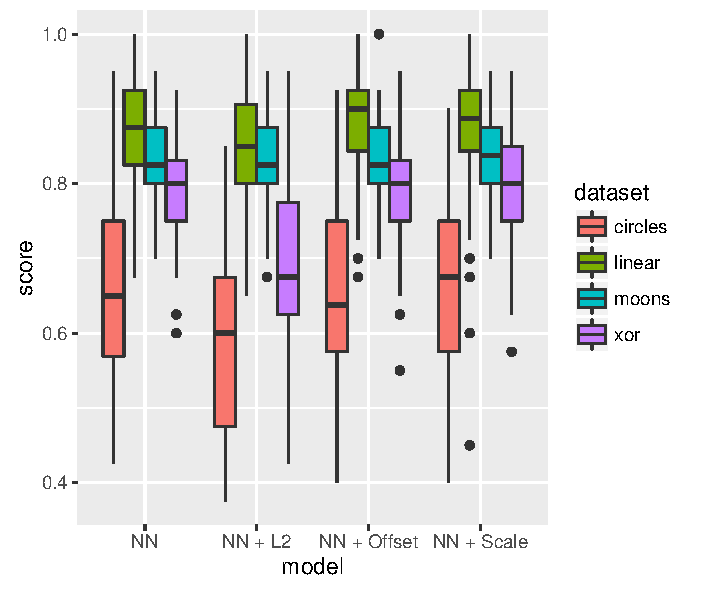
\includegraphics[width=0.5\textwidth]{plots/2d_significant}
	\caption{Boxplot of performance on the 100 datasets for each data generator and classification model.}
\end{figure}

In order to test whether weight decay has an significant improvement to the performance, an independent two-sampled t-test is used (assumes equal variance) on the misclassification rates obtained from the $5$-fold cross-validation for different weight decay parameter values seen in \cref{fig:reg_opt}.

\begin{figure}[H]
  \centering
  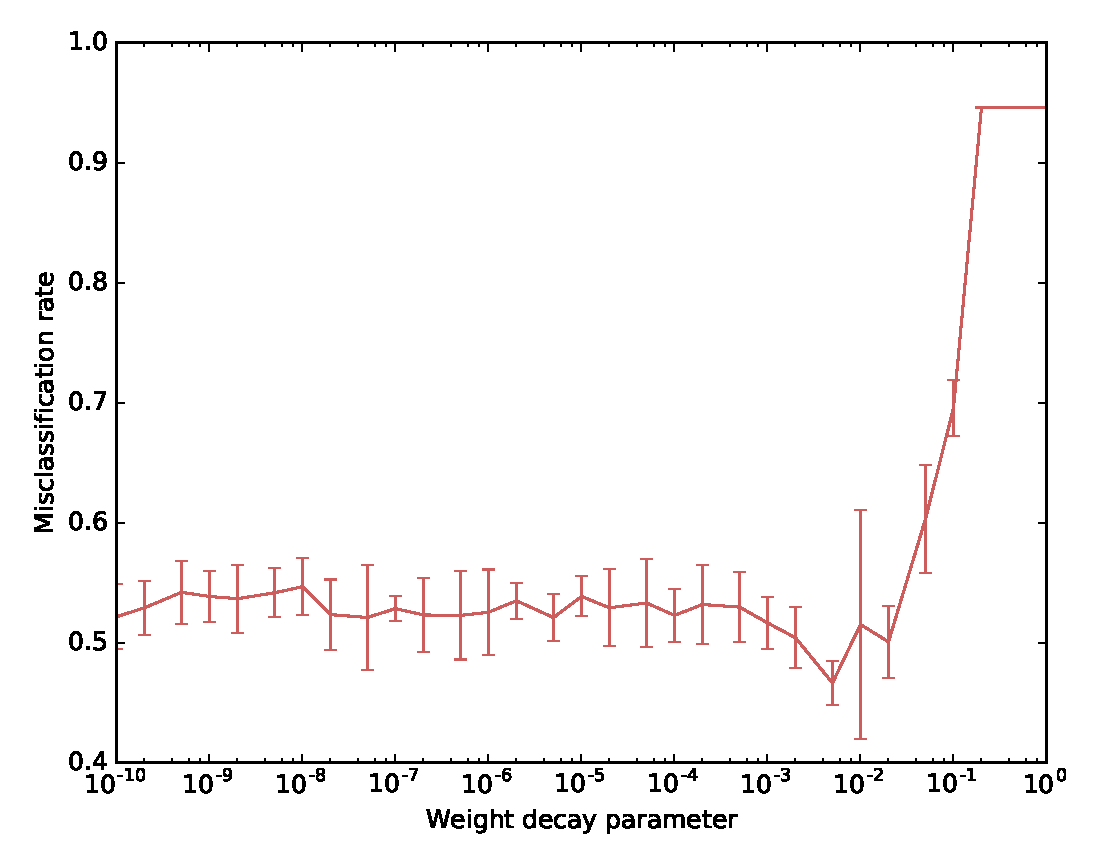
\includegraphics[width=0.4\textwidth]{plots/reg_opt_dieleman_speaker_elsdsr}
  \caption{Misclassification rate confidence interval for different weight decay parameter values, for the speaker classification problem on the ELSDSR dataset, obtained using $5$-fold cross-validation.}
  \label{fig:reg_opt}
\end{figure}

Given the mean misclassification rates $\mu_1$ and $\mu_2$ for the regularization parameter being $0$ and $5 \cdot 10^{-3}$ respectively, our null-hypothesis is defined as $\mu_1$ and $\mu_2$ being different
\begin{equation}
\begin{aligned}
\text{H}_\text{0} \, &\text{:} \, \mu_1 \ne \mu_2 \\
\text{H}_\text{a} \, &\text{:} \, \mu_1 = \mu_2.
\end{aligned}
\end{equation}
The resulting p-value for a two-sided t-test is $p = 0.0030$ i.e. the null-hypothesis is rejected and our alternative hypothesis is confirmed, hence we cannot say that adding weight decay has significant performance improvement with a $95\%$ significance level.


•Objective presentation of key results, without interpretation (text and tables
and figures)
•Important negative results should also be reported

%!TEX root = main.tex
\section{Discussion}
\subsection{TIMIT \& ELSDR}
In the sex classification case (\cref{tab:results-sex}) it is seen that the network models perform better than the GMM on MFCC for both TIMIT and ELSDSR. This is not surprising for the Dieleman models, as they should be able to learn features similar or better than the MFCC features. However, the logistic regression model also performs better. Perhaps this is expected as sex classification do not require a lot of information and thus mean frequencies may suffice. Finally, the logistic regression learns using all observations simultaneously while GMM learns from just one sex at a time which could be an attributing factor for the performance difference.

In the speaker classification case (\cref{tab:results-speaker}) the GMM also performs worse than logistic regression, though in the ELSDSR case it is not significant. This is more surprising as speaker classification should be a much harder problem and thus require a larger feature space. However, this does not appear to be the case. Finally, the Dieleman model performs significantly worse than logistic regression which is the most surprising result. At the very least, one would expect the Dieleman model to be able to learn something similar to the logistic regression. This could suggest that there may be a vanishing moment problem, however, the network is able to overfit and the output distribution of the individual layers don't support this hypothesis. It is also possible that that not enough observations per speaker were available for a CNN to be applicable.

Of all the different regularizations which were tried, the only one which slightly improved the Dieleman model was weight decay. In the original Dieleman paper \cite{dieleman} it was found that weight decay did not improve the performance. We suspect it may also be the case for our problem since our weight decay optimization contains 27 choices ($\lambda \in [10^{-10}, 5 \cdot 10^{-2}]$). Thus with a $95\%$ confidence interval we can expect $1.35$ of those tests to be a type 1 error (false rejection). We suspect that $\lambda = 5 \cdot 10^{-3}$ may be a false rejection.

\subsection{Generated datasets}
Rather surprisingly no instances were found where adding an invariance regularization improved performance. For instance, it was expected that the network would perform better with scale invariance on the xor-dataset because any point should be scalable and still be the same class (not accounting the noise). However, as seen from \cref{fig:reg_opt} and \cref{appendix:generated-contour-optimized} the regularizers do not appear to have any effect.

If one chooses extreme regularization parameters the contours do change as expected. In \cref{plt:generated-contour-extream} this is very apparent for the offset invariant regularizer that prefers contour lines going from bottom left to top right. The scale invariant regularizer also performs very poorly on the circles dataset which is expected seeing as it is the scale that creates the boundary.

An explanation for the poor performance may be the choice of the class outputs in the penalty term ($C_{i,k}$). In this paper, for each observation the output-neuron matching the target class $t$ was chosen (i.e. $k=$t). One could argue that if the network is errorneously giving the target class a low probability then the derivate might also be low. Some experiments were made using the output-neuron with maximum activation ($\max_k C_{i,k} \forall i$) but it did not seem to make a difference.

%!TEX root = main.tex
\section{Conclusion}

In this paper it was shown that the end-to-end learning offered by a Deep convolutional Neural Network performs sex-classification on sound better than using hand-crafted MFCC features and a GMM. However, for speaker-classification logistic regression performed best, which may indicate that a bigger dataset is needed for the DNN. Different types of regularization were added but none improved the results.

Among the regularization methods tried were a new implementation of ``invariance'' regularizers. These were implemented in Theano and in addition to the aforementioned problems it was also evaluated on synthetic datasets. No evidence was found that this form of regularization improved performance on any of the datasets.
%!TEX root = main.tex
\section{Acknowledgement}

•Thank you to people or organizations which made the work possible

\printbibliography

\appendix
%!TEX root = main.tex

\onecolumn
\section{Regularization optimization on generated datasets}
\label{appendix:regualization-optimization}
\begin{figure}[H]
	\centering
	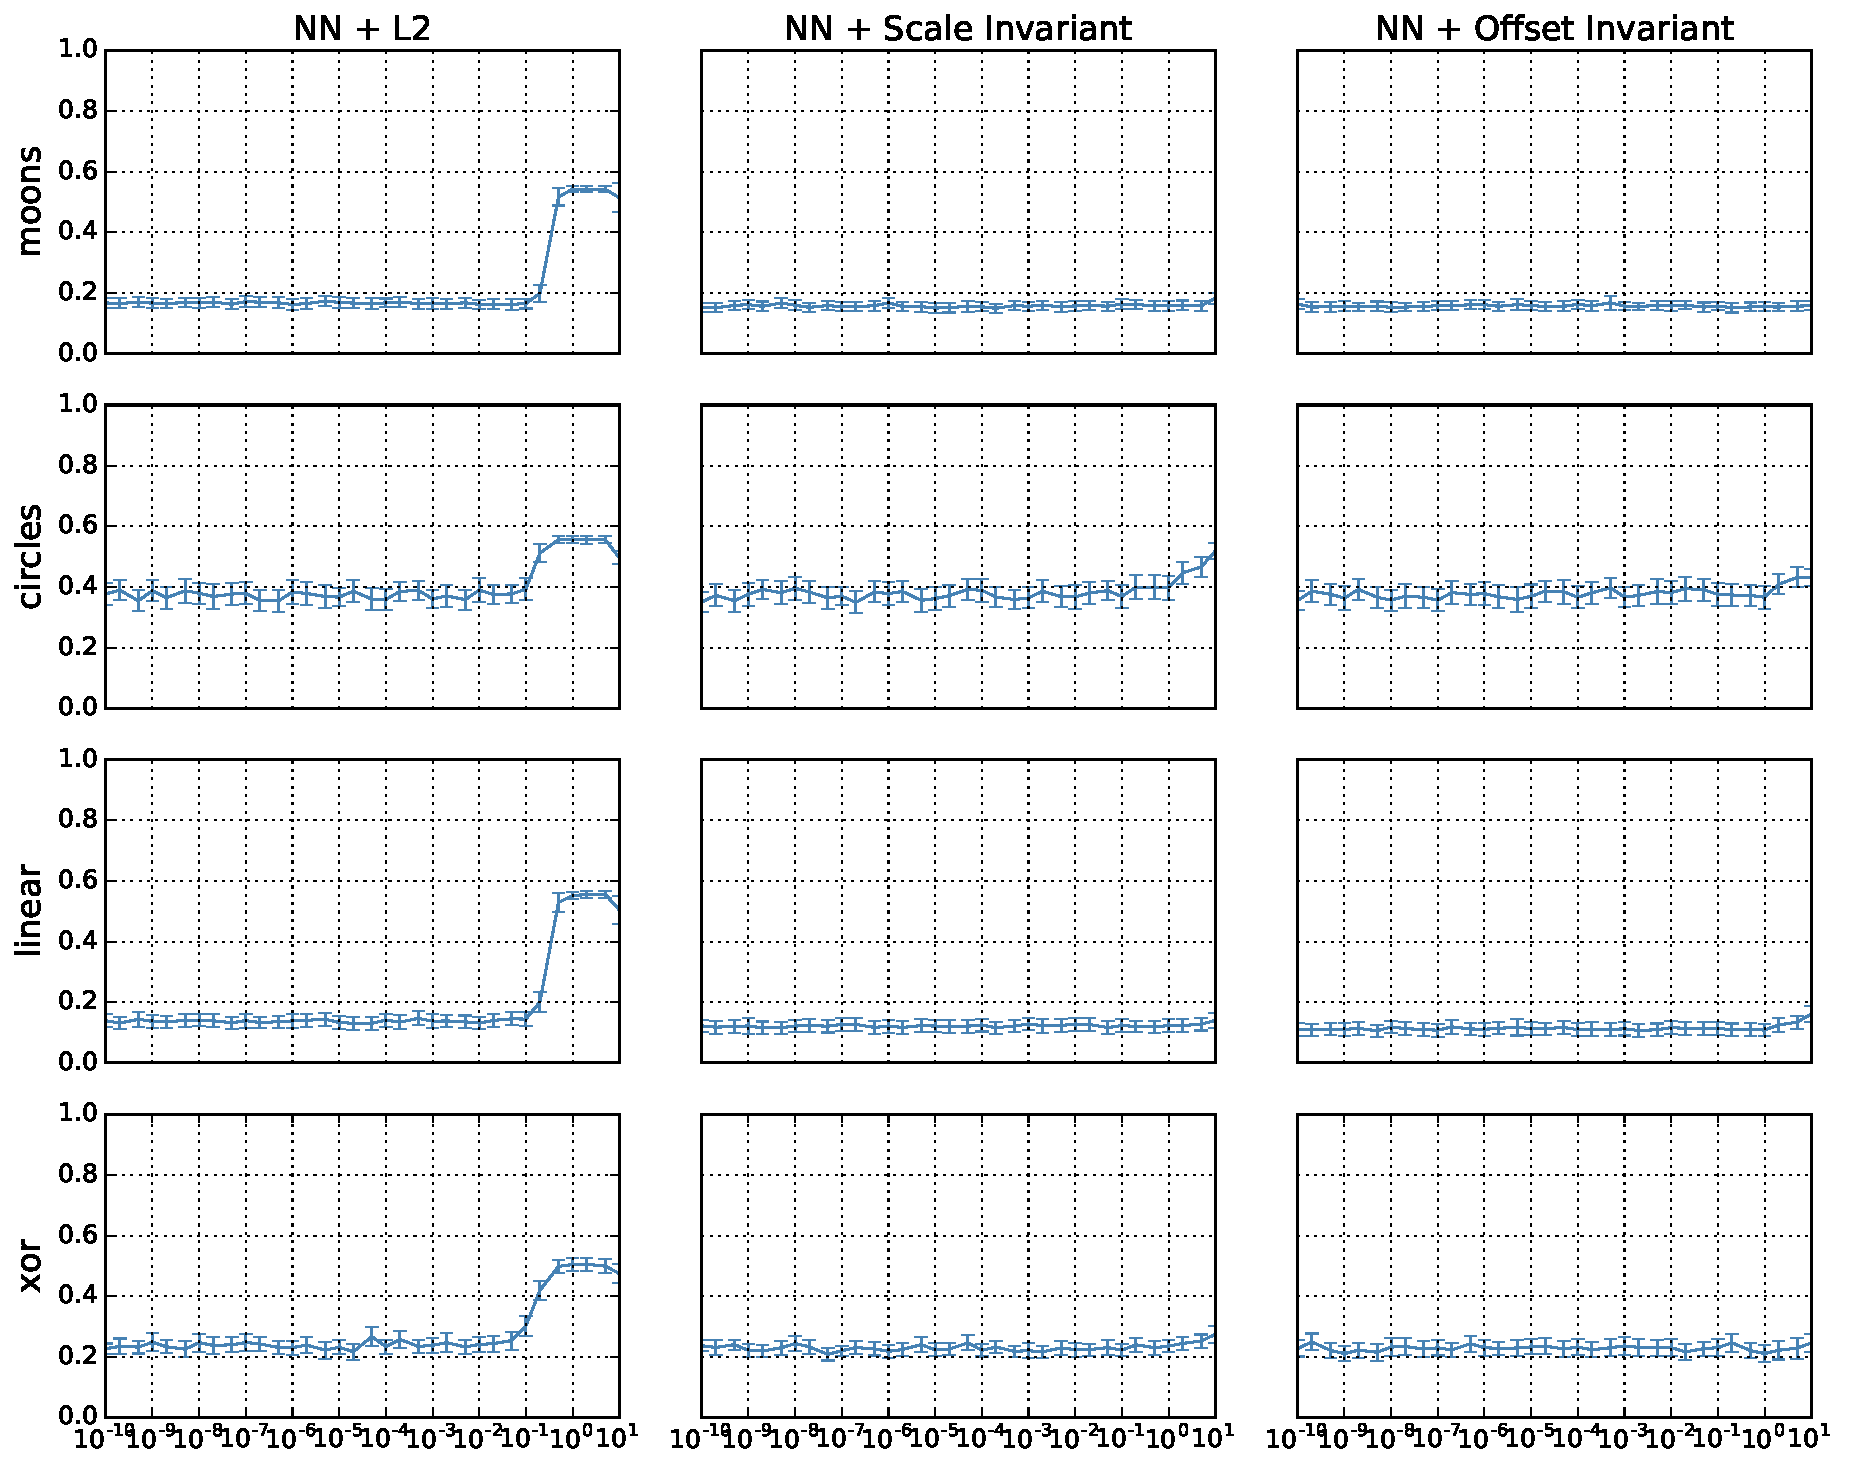
\includegraphics[width=0.7\textwidth]{plots/syntetic_reg_opt}
	\caption{Observations and contour plot of the class probability function for each classifier and dataset.}
\end{figure}

\section{Contour with optimized regularization choices.}
\label{appendix:generated-contour-optimized}
\begin{figure}[H]
	\centering
	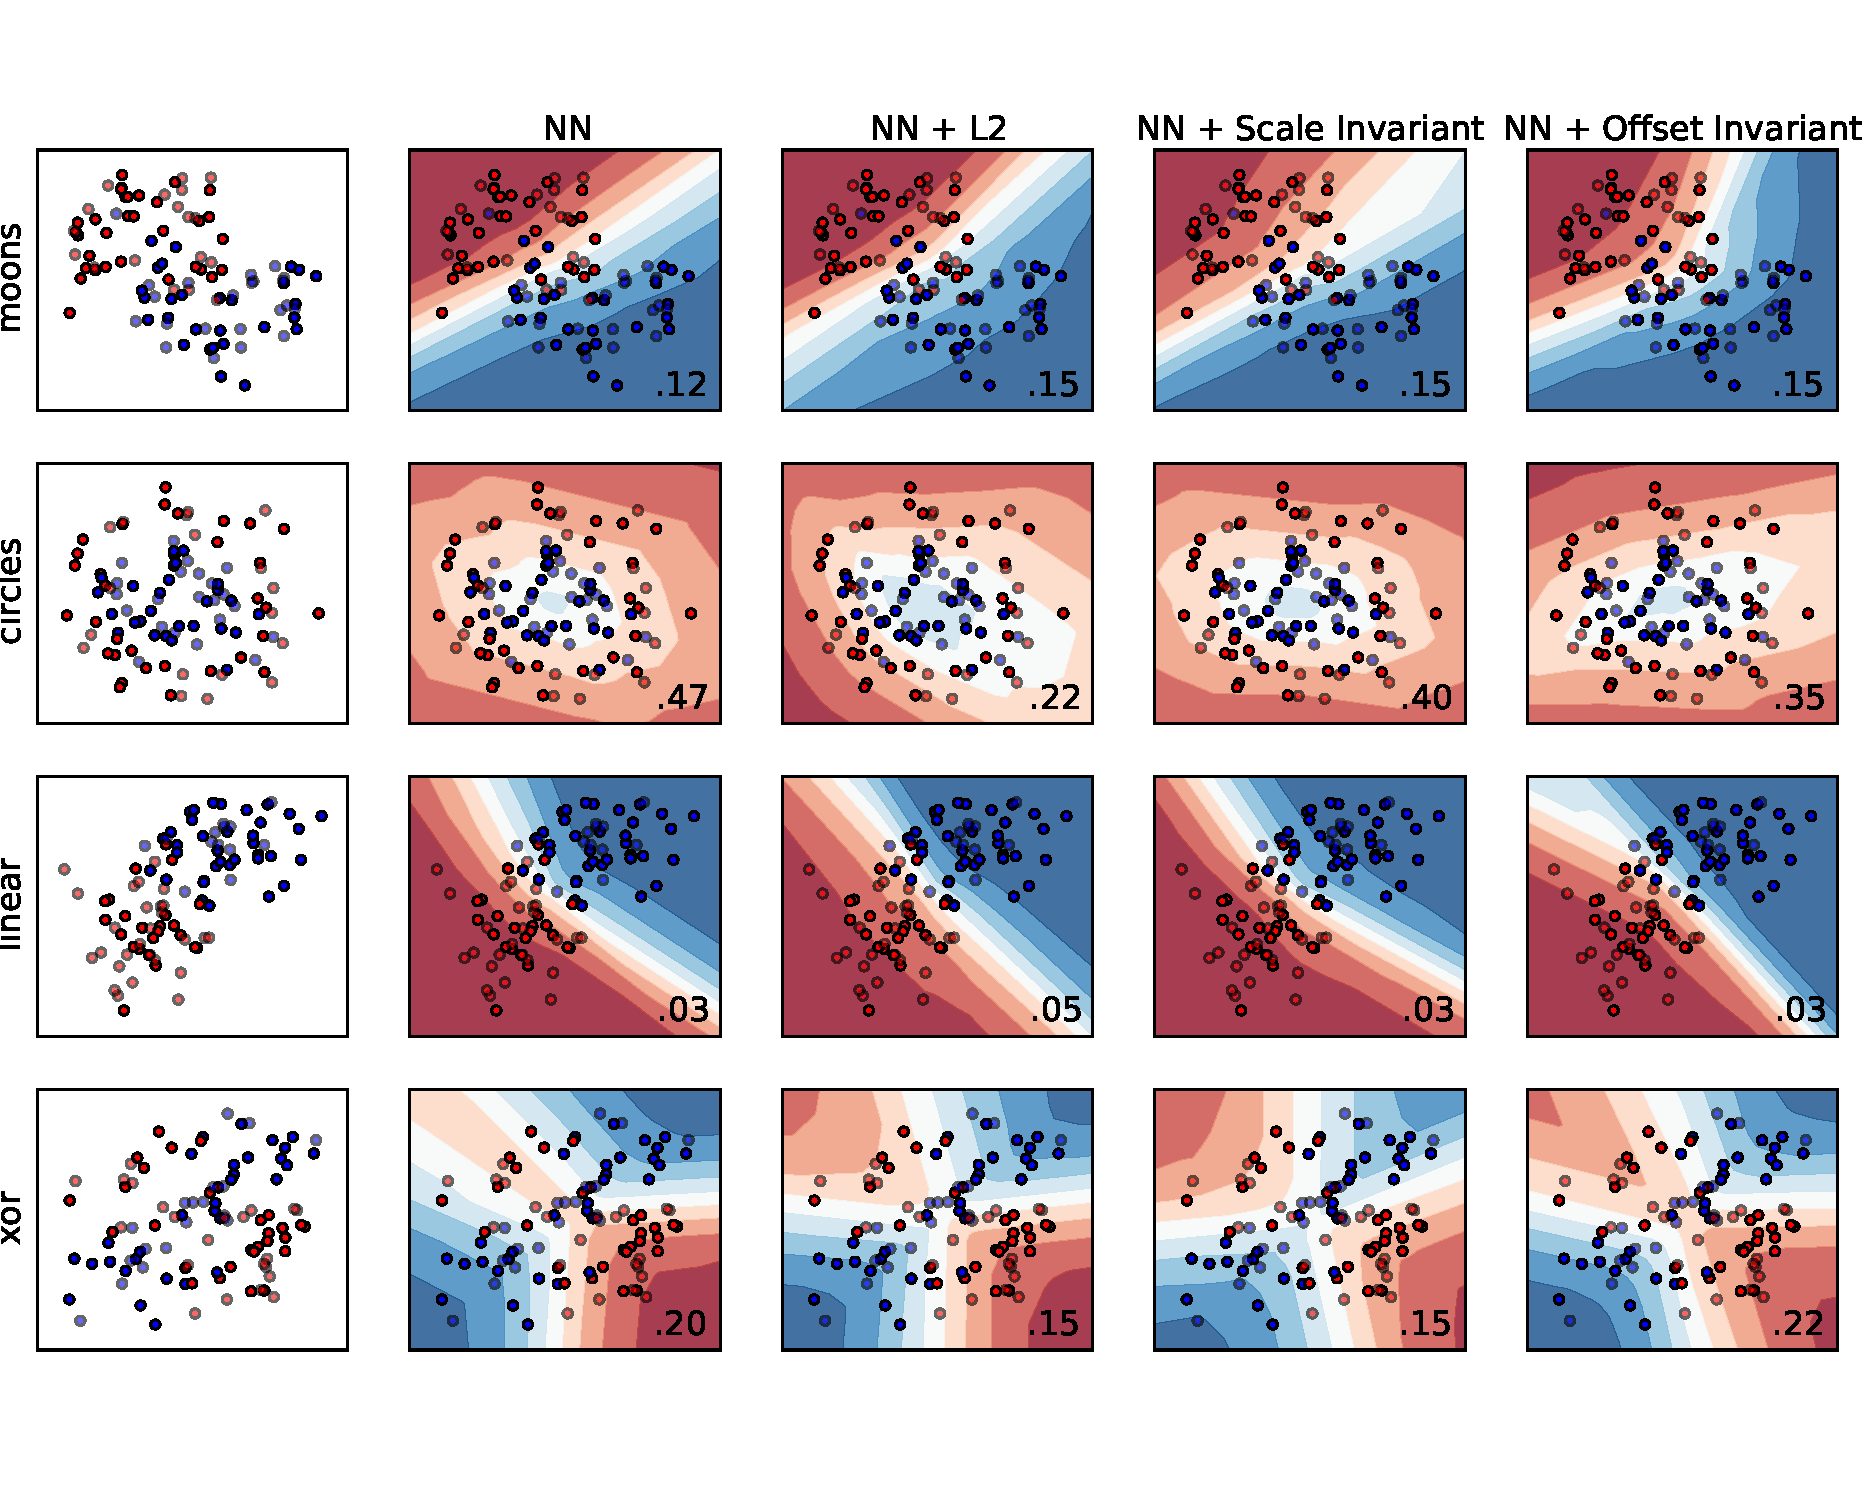
\includegraphics[width=0.7\textwidth, trim = 0 2.2cm 0 1.5cm, clip]{plots/2d_classifier-optimized}
	\caption{Contour plot of the class probability function for each classifier and dataset using optimal regularization choices.}
\end{figure}

\twocolumn
\section{Weekly log}

\section{Week 4}

\subsection{Notes from meeting}

\begin{itemize}
\item What are our ambitions?
\item Neural networks are easy -> done next time
\item Neural networks are dark magic. Not very scientific approach.
\item Is it hard to predict notes from given audio data?
\end{itemize}

\subsection{For next meeting}

\textbf{Next meeting on March 1st}

\begin{itemize}
\item Read articles provided by Bjørn
\end{itemize}


\section{Week 5}

\subsection{Notes from meeting}

\begin{itemize}
\item The \textit{Sander Dieleman} article ``end-to-end learning for music
audio'' should be a good starting point.
\item Use the \texttt{timit} dataset for classification.
\item ``sensitivitet regulization'' is an interesting project direction
\item We should consider what is relevant to be invariant about. In pictures
rotational or translation invariance might make sense.
\end{itemize}

\subsection{For next meeting}

\textbf{Next meeting on March 10.}

\begin{itemize}
\item Write resume of the ``end-to-end learning for music audio'' paper.
\item Try implementing basic classification using timit data. (internal
agreement)
\end{itemize}


\subsection{Week 6}

\subsubsection{Notes from meeting}

\begin{itemize}
\item The number of bins used in our spectogram calculations are too few -> use twice the amount (approx. $100$Hz).
\item What should we do about variable input size? (length of sound files varies)
\item Too large learning rate could be a problem for converging.
\item Initialization of weights can be a major factor in convergance/performance of a network. If we want to look into steps that can be used for initializing these in a proper way, we can take a look at the 5-step process described in Jan's PhD.
\end{itemize}

\subsubsection{For next meeting}

\begin{itemize}
\item Next meeting on March 17th
\item Look into solutions to variable input size.
\item Implement CV, i.e. validate predictions
\item Normalize the input, e.g. $\log$ of spectogram (or energy/RMS-normalization)
\item Maybe add some form of regularization to the network
\end{itemize}


\section{Week 7}

\subsection{Notes from meeting}

\begin{itemize}
\item RMS-normalization of raw audio signals could be a good idea.
\item Robustness of model -> Add ``soft'' invariance regularization terms to cost function (Bjørn will be happy if we can implement this at some point).
\item A linear model using the spectrograms can be used as benchmark.
\item The book ``Digital Speech Processing'' has a section about Mel-spectrogram we can look at (not important).
\item A custom pooling layer could be a solution to varying input size.
\end{itemize}

\subsection{For next meeting}

\textbf{Next meeting on March 31th}

\begin{itemize}
\item Compare with the simple linear model.
\item Itemwise RMS normalization.
\item Think about what the model should be invariant of.
\item Look at the variance of the network output before training.
\end{itemize}


\section{Week 8}

\subsection{Notes from meeting}

\begin{itemize}
\item
\end{itemize}

\subsection{For next meeting}

\textbf{Next meeting on April 7th}

\begin{itemize}
\item
\end{itemize}


\section{Week 9}

\subsection{Notes from meeting}

\begin{itemize}
\item Sex classification is too easy a problem. Try speaker classification.
\item What tranformation function $s(x, \alpha)$ makes sense to be invariant to.
\item Transformations could be
\begin{itemize}
  \item Pitch shift
  \item Hoarse voice
  \item Noise
  \item Filter (e.g. \textit{low-pass})
\end{itemize}
\item No free lunch theorem.
\end{itemize}

\subsection{For next meeting}

\textbf{Next meeting on April 14th}

\begin{itemize}
\item Try classifying speakers instead of sex.
\item Look at audio degredation toolbox as tranformation function we want the network to be invariant to.
\item Try to implement the explicit tranformation invariance term to the loss function.
\end{itemize}


\section{Week 10}

\subsection{Notes from meeting}

\begin{itemize}
\item Create our own dataset of speakers represented $x$ number of times.
\item Make sure to cross validate the errors, when the final results are being made.
\item Could the performance of the speaker classifier be compared with human
performance?
\item The ELSDSR dataset could be used for speaker classification instead of the Timit.
\end{itemize}

\subsection{For next meeting}

\textbf{Next meeting on April 21th}

\begin{itemize}
\item Send code of invariance implementation to Bjørn. Write details of preprocessing used etc.
\item Regularize network for speaker classification. Try weight decay and dropout.
\item Test the invariance implementation on simple problem from UCI with a simple network before testing on Dieleman.
\item Reduce number of speakers used. E.g. only include speakers represented 10 times or more in the dataset.
\end{itemize}


\subsection{Week 11}

\subsubsection{Notes from meeting}

\begin{itemize}
\item $80-90 \%$ correct classification rate should be possible for speaker classifier.
\item Mean spectrogram with logitic regression.
\item Does the size on the dense layer limit our network? 300 output neurons vs 50 neurons in last dense layer??
\end{itemize}

\subsubsection{For next meeting}

\begin{itemize}
\item Next meeting on April 28th
\item Give Bjørn the data for speaker classification.
\item Give Bjørn access to github repository - maybe make it public.
\item Try mean spectogram on frequency axis using simple logistic regression.
\item Try binary classification - 1 vs many on speaker classification.
\end{itemize}


\subsection{Week 12}

\subsubsection{Notes from meeting}

\begin{itemize}
\item Bjørn will stop being our supervisor
\item We could not get any improvement over logistic regression by applying convolution. This should not be.
\item Trying another dataset showed the same behaviour.
\end{itemize}

\subsubsection{For next meeting}

\begin{itemize}
\item Next meeting on ``not agreed''
\item We should try a GMM model as a baseline
\item Bjørn will also try calculating a baseline
\item Look at Jan \& Corey paper to get baseline
\end{itemize}


\subsection{Week 13}

\subsubsection{Notes from meeting}

\begin{itemize}
\item Poster for the presentation should be made as a A0 paper.
\item The examiner will be allowed to ask into any topic mentioned in the presentation (including MFCC features).
\item We should think of an explanation for why Weight Decay isn't improving performance.
\item The structure of the representation should match the structure of the report. Explain from beginning to end in a coherent manner.
\end{itemize}



\end{document}
